Let the equation of line be
\begin{align}
    \vec{n}^\top\brak{\vec{x}-\vec{P}}=0
\end{align}
So the perpendicular from the origin meets the line at $\vec{P}= \myvec{-2 \\ 9}$.Since,
\begin{align}
   \vec{n}&= \vec{P}-\vec{O}\\
   &=\myvec{-2-0\\9-0}\\
   &=\myvec{-2\\9}
\end{align}
is the normal vector where $\vec{O}$ is the origin then 
is the direction vector, Hence the equation of line is given by
\begin{align}
   \myvec{-2 & 9}\brak{\vec{x}-\myvec{-2 \\ 9}}&=0 \\
\implies     \myvec{-2 & 9}\vec{x}&= 85
\end{align}
    See Fig. \ref{aug/2/21/fig:my_label}
\begin{figure}[htp]
    \centering
    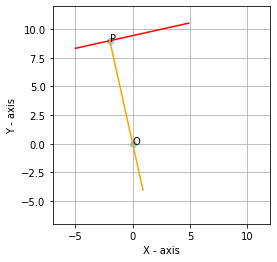
\includegraphics{solutions/aug/2/21/Assignment_4.png}
    \caption{graph}
    \label{aug/2/21/fig:my_label}
\end{figure}

